\documentclass[10pt]{beamer}
\usetheme{default}
\usepackage[utf8]{inputenc}
\usepackage{graphicx}
\usepackage{booktabs}
\title{Bina.az Price Prediction: From-Scratch Trees and a Pegasos SVM}
\author{Shukurlu, Nural \hspace{1em} MLE-AI-201, AI Academy}
\date{October 2026}
\begin{document}
\frame{\titlepage}

\begin{frame}{Problem and data}
\begin{itemize}
\item Task A: predict sale price (trained on $\log(\mathrm{price})$).
\item Task B: premium vs.\ standard tier at train median 213{,}000~AZN.
\item 100{,}775 raw rows $\to$ 62{,}673 clean, 43 features, split 43869/9402/9402.
\end{itemize}
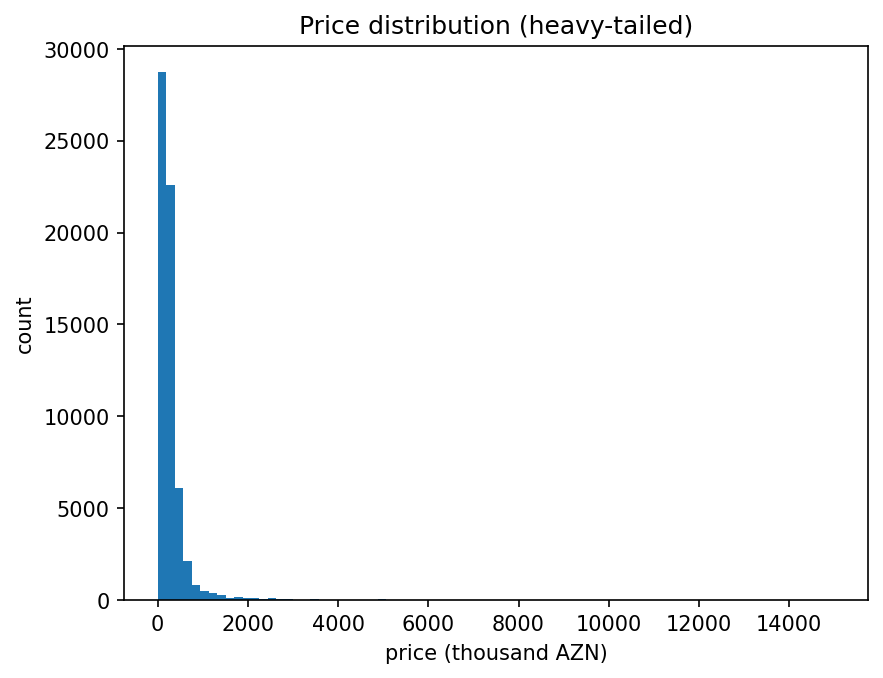
\includegraphics[width=\linewidth,height=0.5\textheight,keepaspectratio]{../report/figures/price_hist.png}
\end{frame}

\begin{frame}{Cleaning and leakage}
\begin{itemize}
\item Dedup on listing URL; parsed area, floors (``7~/~9''), land (sot).
\item Dropped price/area outliers and off-map coordinates; all prices AZN.
\item Removed \texttt{unit\_price}, \texttt{total\_price} (== price) + IDs, URLs, names, free text.
\item Threshold and scaling statistics from train only.
\end{itemize}
\end{frame}

\begin{frame}{Decision tree (from scratch)}
\begin{itemize}
\item Gini / entropy / MSE, exact split search, depth/leaf/impurity stops.
\item Task A: best depth 12, leaf 5. Task B: Gini 0.918 beats entropy 0.916.
\end{itemize}
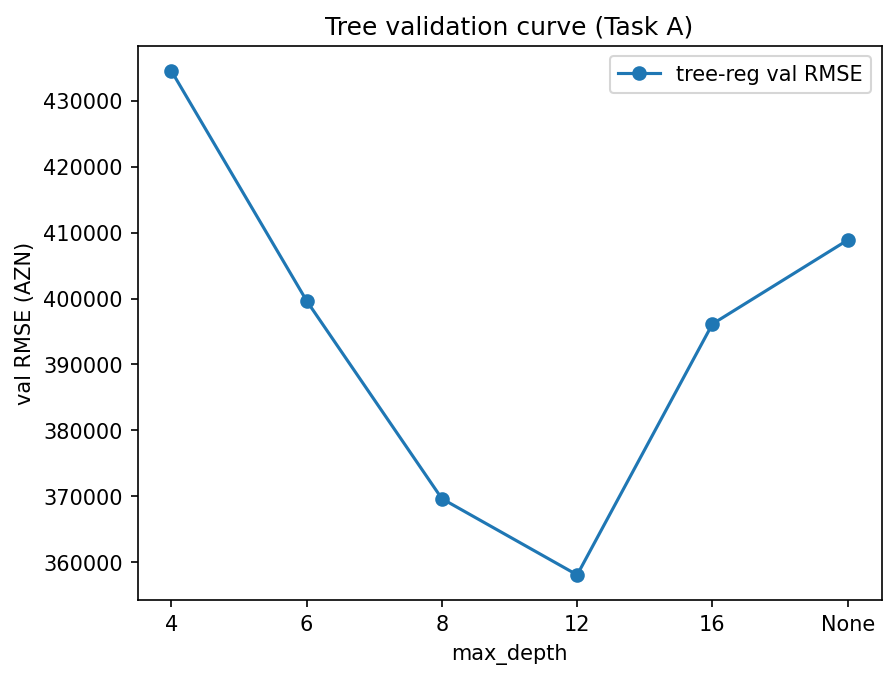
\includegraphics[width=\linewidth,height=0.55\textheight,keepaspectratio]{../report/figures/tree_val_curve.png}
\end{frame}

\begin{frame}{Pegasos SVM (from scratch)}
\begin{itemize}
\item $J(w,b)=\frac{\lambda}{2}\|w\|^2+\frac{1}{n}\sum\max(0,1-y_i(w^Tx_i+b))$, $\eta_t=1/(\lambda t)$.
\item Best $\lambda=0.01$: margin 0.73, support fraction 0.40, val F1 0.832.
\item RFF extension ($D{=}500$) tried, trails linear (0.767): linear kept.
\end{itemize}
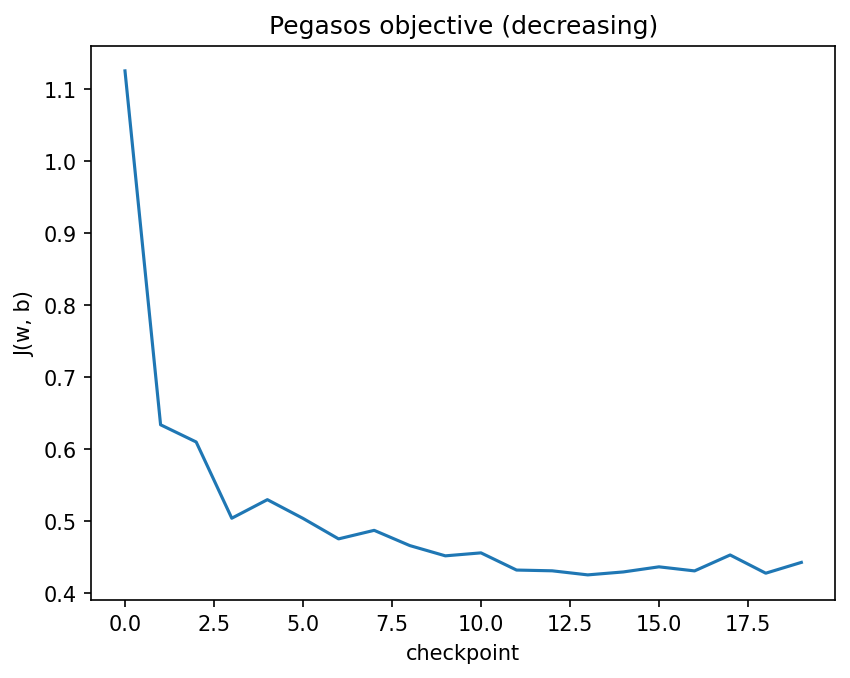
\includegraphics[width=\linewidth,height=0.42\textheight,keepaspectratio]{../report/figures/svm_objective.png}
\end{frame}

\begin{frame}{Results}
\begin{tabular}{@{}lcc@{}}
\toprule Model & Task A RMSE & Task B F1 \\
\midrule My tree & 368{,}435 & 0.918 \\
sklearn tree & 377{,}891 & 0.919 \\
My SVM & --- & 0.832 \\
sklearn SGD & --- & 0.854 \\
\bottomrule
\end{tabular}
\begin{itemize}
\item Test: tree $R^2$ 0.55, AUC 0.955; SVM AUC 0.920. CV: $0.911{\pm}0.002$ / $0.832{\pm}0.007$.
\item One command reproduces all: \texttt{python -m src.run\_all}.
\end{itemize}
\end{frame}

\begin{frame}{What drives predictions}
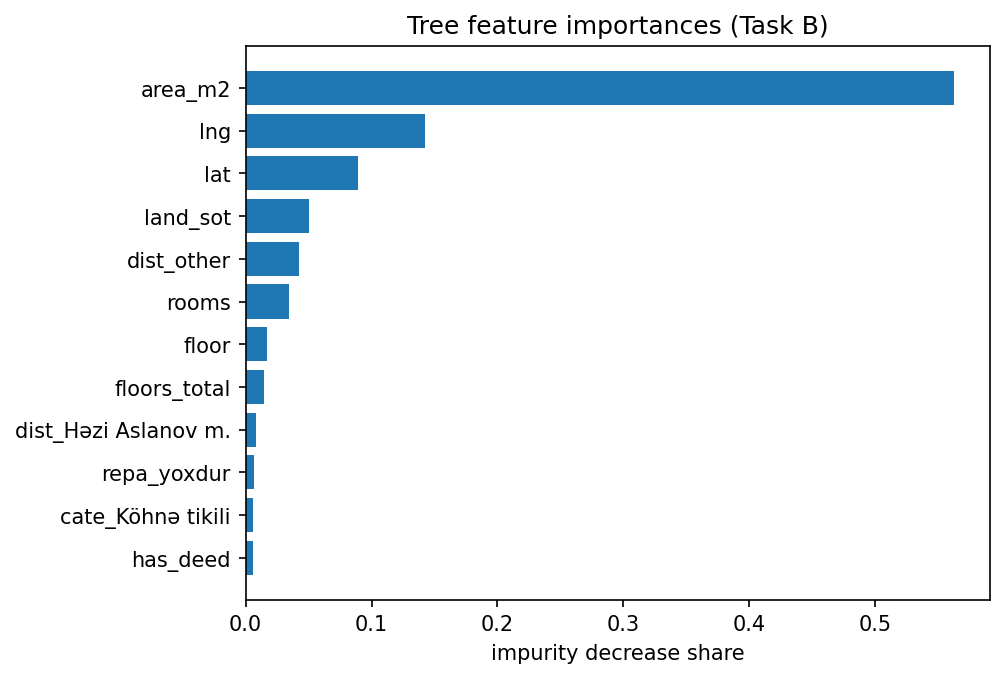
\includegraphics[width=\linewidth,height=0.55\textheight,keepaspectratio]{../report/figures/importance.png}
Area, district and rooms dominate; deed/repair flags help at the margin.
\end{frame}

\begin{frame}{Where models fail}
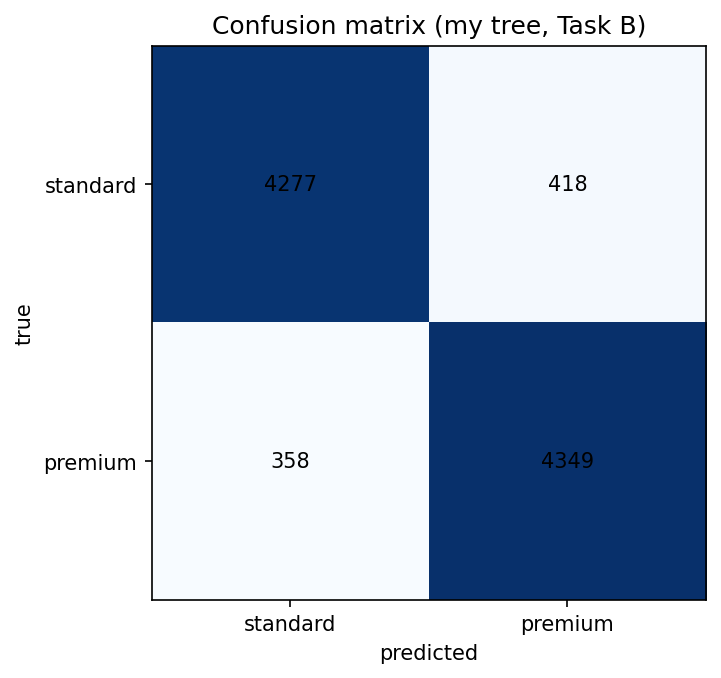
\includegraphics[width=0.55\linewidth,height=0.5\textheight,keepaspectratio]{../report/figures/confusion.png}
\begin{itemize}
\item Luxury outliers inflate RMSE (MAE only 86k); sparse outskirt districts are thin.
\item Single split headline + train-only CV; no text/image features yet.
\end{itemize}
\end{frame}

\begin{frame}{Next steps}
\begin{itemize}
\item Description-text features and district-grouped error modelling.
\item Contributions: see \texttt{contribution\_report.md} in the repo root.
\item Repo: \texttt{github.com/nuralnetworks/bina-az-price-prediction} (tag \texttt{v1.0-final}); report + this deck submitted on Moodle.
\end{itemize}
\end{frame}
\end{document}
